% Created by tikzDevice version 0.12.6 on 2024-08-15 14:32:08
% !TEX encoding = UTF-8 Unicode
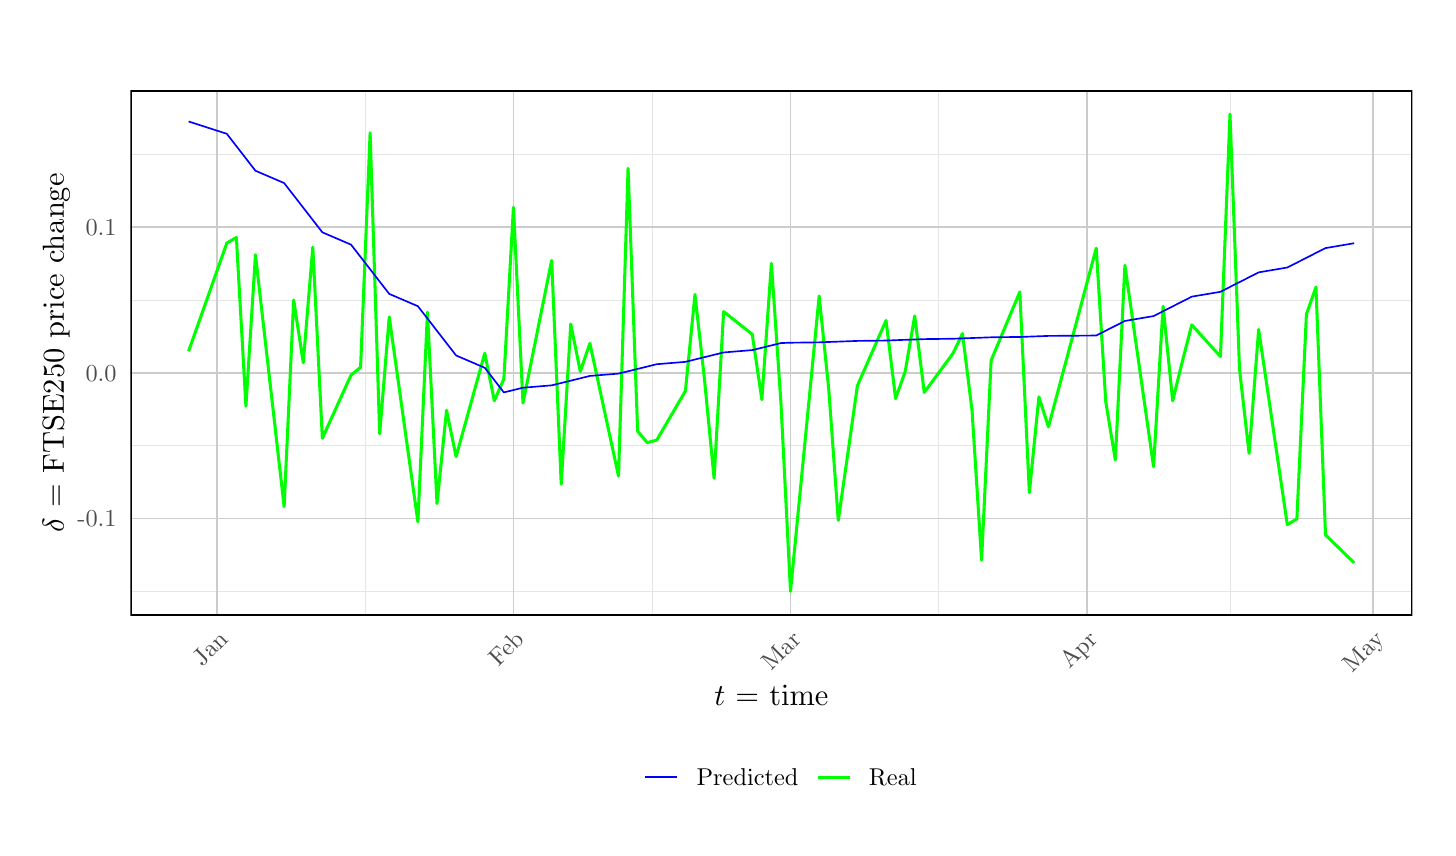
\begin{tikzpicture}[x=1pt,y=1pt]
\definecolor{fillColor}{RGB}{255,255,255}
\path[use as bounding box,fill=fillColor,fill opacity=0.00] (0,0) rectangle (505.89,289.08);
\begin{scope}
\path[clip] ( 37.09, 76.79) rectangle (500.39,266.42);
\definecolor{drawColor}{gray}{0.90}

\path[draw=drawColor,line width= 0.3pt,line join=round] ( 37.09, 85.39) --
	(500.39, 85.39);

\path[draw=drawColor,line width= 0.3pt,line join=round] ( 37.09,138.04) --
	(500.39,138.04);

\path[draw=drawColor,line width= 0.3pt,line join=round] ( 37.09,190.69) --
	(500.39,190.69);

\path[draw=drawColor,line width= 0.3pt,line join=round] ( 37.09,243.34) --
	(500.39,243.34);

\path[draw=drawColor,line width= 0.3pt,line join=round] (122.02, 76.79) --
	(122.02,266.42);

\path[draw=drawColor,line width= 0.3pt,line join=round] (225.59, 76.79) --
	(225.59,266.42);

\path[draw=drawColor,line width= 0.3pt,line join=round] (329.15, 76.79) --
	(329.15,266.42);

\path[draw=drawColor,line width= 0.3pt,line join=round] (434.45, 76.79) --
	(434.45,266.42);
\definecolor{drawColor}{gray}{0.80}

\path[draw=drawColor,line width= 0.6pt,line join=round] ( 37.09,111.72) --
	(500.39,111.72);

\path[draw=drawColor,line width= 0.6pt,line join=round] ( 37.09,164.37) --
	(500.39,164.37);

\path[draw=drawColor,line width= 0.6pt,line join=round] ( 37.09,217.02) --
	(500.39,217.02);

\path[draw=drawColor,line width= 0.6pt,line join=round] ( 68.50, 76.79) --
	( 68.50,266.42);

\path[draw=drawColor,line width= 0.6pt,line join=round] (175.53, 76.79) --
	(175.53,266.42);

\path[draw=drawColor,line width= 0.6pt,line join=round] (275.64, 76.79) --
	(275.64,266.42);

\path[draw=drawColor,line width= 0.6pt,line join=round] (382.67, 76.79) --
	(382.67,266.42);

\path[draw=drawColor,line width= 0.6pt,line join=round] (486.24, 76.79) --
	(486.24,266.42);
\definecolor{drawColor}{RGB}{0,255,0}

\path[draw=drawColor,line width= 1.1pt,line join=round] ( 58.15,172.17) --
	( 71.96,211.24) --
	( 75.41,213.25) --
	( 78.86,152.32) --
	( 82.31,207.00) --
	( 92.67,116.02) --
	( 96.12,190.68) --
	( 99.58,168.03) --
	(103.03,209.77) --
	(106.48,140.72) --
	(116.84,163.52) --
	(120.29,166.35) --
	(123.74,251.08) --
	(127.19,142.33) --
	(130.65,184.56) --
	(141.00,110.53) --
	(144.46,186.25) --
	(147.91,117.15) --
	(151.36,150.82) --
	(154.81,134.08) --
	(165.17,171.43) --
	(168.62,154.27) --
	(172.07,162.13) --
	(175.53,224.16) --
	(178.98,153.45) --
	(189.34,204.97) --
	(192.79,124.11) --
	(196.24,181.98) --
	(199.69,164.84) --
	(203.15,175.02) --
	(213.50,127.04) --
	(216.95,238.21) --
	(220.41,143.25) --
	(223.86,139.14) --
	(227.31,140.03) --
	(237.67,157.78) --
	(241.12,192.66) --
	(244.57,161.89) --
	(248.03,126.27) --
	(251.48,186.49) --
	(261.83,178.26) --
	(265.29,154.67) --
	(268.74,203.94) --
	(272.19,153.48) --
	(275.64, 85.41) --
	(286.00,192.13) --
	(289.45,158.59) --
	(292.91,111.06) --
	(296.36,135.16) --
	(299.81,159.67) --
	(310.17,183.27) --
	(313.62,155.11) --
	(317.07,164.71) --
	(320.52,184.91) --
	(323.98,157.28) --
	(334.33,171.33) --
	(337.79,178.53) --
	(341.24,150.76) --
	(344.69, 96.64) --
	(348.14,168.85) --
	(358.50,193.58) --
	(361.95,121.10) --
	(365.40,155.64) --
	(368.86,144.86) --
	(386.12,209.40) --
	(389.57,153.90) --
	(393.02,132.84) --
	(396.48,203.20) --
	(406.83,130.44) --
	(410.28,188.41) --
	(413.74,154.24) --
	(417.19,168.30) --
	(420.64,181.69) --
	(431.00,170.25) --
	(434.45,257.80) --
	(437.90,165.53) --
	(441.36,135.21) --
	(444.81,180.03) --
	(455.16,109.50) --
	(458.62,111.56) --
	(462.07,185.54) --
	(465.52,195.32) --
	(468.97,105.79) --
	(479.33, 95.66);
\definecolor{drawColor}{RGB}{0,0,255}

\path[draw=drawColor,line width= 0.6pt,line join=round] ( 58.15,255.18) --
	( 71.96,250.73) --
	( 75.41,246.28) --
	( 78.86,241.83) --
	( 82.31,237.38) --
	( 92.67,232.93) --
	( 96.12,228.48) --
	( 99.58,224.03) --
	(103.03,219.58) --
	(106.48,215.13) --
	(116.84,210.68) --
	(120.29,206.23) --
	(123.74,201.78) --
	(127.19,197.33) --
	(130.65,192.88) --
	(141.00,188.43) --
	(144.46,183.98) --
	(147.91,179.53) --
	(151.36,175.08) --
	(154.81,170.63) --
	(165.17,166.18) --
	(168.62,161.73) --
	(172.07,157.28) --
	(175.53,158.13) --
	(178.98,158.98) --
	(189.34,159.83) --
	(192.79,160.68) --
	(196.24,161.53) --
	(199.69,162.38) --
	(203.15,163.23) --
	(213.50,164.08) --
	(216.95,164.92) --
	(220.41,165.77) --
	(223.86,166.62) --
	(227.31,167.47) --
	(237.67,168.32) --
	(241.12,169.17) --
	(244.57,170.02) --
	(248.03,170.87) --
	(251.48,171.72) --
	(261.83,172.57) --
	(265.29,173.41) --
	(268.74,174.26) --
	(272.19,175.11) --
	(275.64,175.24) --
	(286.00,175.37) --
	(289.45,175.50) --
	(292.91,175.63) --
	(296.36,175.76) --
	(299.81,175.89) --
	(310.17,176.02) --
	(313.62,176.15) --
	(317.07,176.28) --
	(320.52,176.41) --
	(323.98,176.54) --
	(334.33,176.67) --
	(337.79,176.80) --
	(341.24,176.93) --
	(344.69,177.06) --
	(348.14,177.19) --
	(358.50,177.32) --
	(361.95,177.44) --
	(365.40,177.57) --
	(368.86,177.70) --
	(386.12,177.83) --
	(389.57,179.59) --
	(393.02,181.34) --
	(396.48,183.10) --
	(406.83,184.86) --
	(410.28,186.61) --
	(413.74,188.37) --
	(417.19,190.12) --
	(420.64,191.88) --
	(431.00,193.63) --
	(434.45,195.39) --
	(437.90,197.14) --
	(441.36,198.90) --
	(444.81,200.66) --
	(455.16,202.41) --
	(458.62,204.17) --
	(462.07,205.92) --
	(465.52,207.68) --
	(468.97,209.43) --
	(479.33,211.19);
\definecolor{drawColor}{RGB}{0,0,0}

\path[draw=drawColor,line width= 1.1pt,line join=round,line cap=round] ( 37.09, 76.79) rectangle (500.39,266.42);
\end{scope}
\begin{scope}
\path[clip] (  0.00,  0.00) rectangle (505.89,289.08);
\definecolor{drawColor}{gray}{0.30}

\node[text=drawColor,anchor=base east,inner sep=0pt, outer sep=0pt, scale=  0.88] at ( 32.14,108.69) {-0.1};

\node[text=drawColor,anchor=base east,inner sep=0pt, outer sep=0pt, scale=  0.88] at ( 32.14,161.34) {0.0};

\node[text=drawColor,anchor=base east,inner sep=0pt, outer sep=0pt, scale=  0.88] at ( 32.14,213.99) {0.1};
\end{scope}
\begin{scope}
\path[clip] (  0.00,  0.00) rectangle (505.89,289.08);
\definecolor{drawColor}{gray}{0.30}

\node[text=drawColor,rotate= 45.00,anchor=base east,inner sep=0pt, outer sep=0pt, scale=  0.88] at ( 72.79, 67.55) {Jan};

\node[text=drawColor,rotate= 45.00,anchor=base east,inner sep=0pt, outer sep=0pt, scale=  0.88] at (179.81, 67.55) {Feb};

\node[text=drawColor,rotate= 45.00,anchor=base east,inner sep=0pt, outer sep=0pt, scale=  0.88] at (279.93, 67.55) {Mar};

\node[text=drawColor,rotate= 45.00,anchor=base east,inner sep=0pt, outer sep=0pt, scale=  0.88] at (386.95, 67.55) {Apr};

\node[text=drawColor,rotate= 45.00,anchor=base east,inner sep=0pt, outer sep=0pt, scale=  0.88] at (490.52, 67.55) {May};
\end{scope}
\begin{scope}
\path[clip] (  0.00,  0.00) rectangle (505.89,289.08);
\definecolor{drawColor}{RGB}{0,0,0}

\node[text=drawColor,anchor=base,inner sep=0pt, outer sep=0pt, scale=  1.10] at (268.74, 44.09) {$t$ = time};
\end{scope}
\begin{scope}
\path[clip] (  0.00,  0.00) rectangle (505.89,289.08);
\definecolor{drawColor}{RGB}{0,0,0}

\node[text=drawColor,rotate= 90.00,anchor=base,inner sep=0pt, outer sep=0pt, scale=  1.10] at ( 13.08,171.61) {$\delta$ = FTSE250 price change};
\end{scope}
\begin{scope}
\path[clip] (  0.00,  0.00) rectangle (505.89,289.08);
\definecolor{drawColor}{RGB}{0,0,255}

\path[draw=drawColor,line width= 0.6pt,line join=round] (223.21, 18.23) -- (234.78, 18.23);
\end{scope}
\begin{scope}
\path[clip] (  0.00,  0.00) rectangle (505.89,289.08);
\definecolor{drawColor}{RGB}{0,255,0}

\path[draw=drawColor,line width= 1.1pt,line join=round] (285.47, 18.23) -- (297.04, 18.23);
\end{scope}
\begin{scope}
\path[clip] (  0.00,  0.00) rectangle (505.89,289.08);
\definecolor{drawColor}{RGB}{0,0,0}

\node[text=drawColor,anchor=base west,inner sep=0pt, outer sep=0pt, scale=  0.88] at (241.72, 15.20) {Predicted};
\end{scope}
\begin{scope}
\path[clip] (  0.00,  0.00) rectangle (505.89,289.08);
\definecolor{drawColor}{RGB}{0,0,0}

\node[text=drawColor,anchor=base west,inner sep=0pt, outer sep=0pt, scale=  0.88] at (303.98, 15.20) {Real};
\end{scope}
\end{tikzpicture}
